% Made up for the tikra gallery: a bar chart whose bars you set by hand, and their mean. In the
% playground, drag the top of a bar.
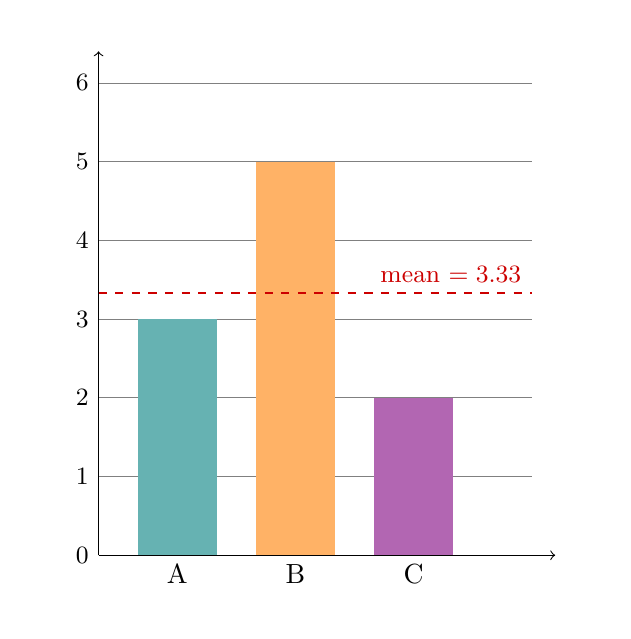
\begin{tikzpicture}
  \def\ba{3}   % first bar, 0..6
  \def\bb{5}   % second bar, 0..6
  \def\bc{2}   % third bar, 0..6
  \useasboundingbox (-0.9,-0.7) rectangle (6.4,6.7);
  \draw[help lines] (0,0) grid[xstep=10, ystep=1] (5.5,6);
  \foreach \y in {0,...,6} \node[left, font=\small] at (0,\y) {\y};
  \draw[->] (0,0) -- (5.8,0);
  \draw[->] (0,0) -- (0,6.4);
  \foreach \v/\x/\c/\name in {\ba/1/teal/A, \bb/2.5/orange/B, \bc/4/violet/C} {
    \fill[\c!60] (\x-0.5,0) rectangle (\x+0.5,\v);
    \node[below] at (\x,0) {\name};
  }
  \coordinate (A) at (1,\ba);
  \coordinate (B) at (2.5,\bb);
  \coordinate (C) at (4,\bc);
  \pgfmathsetmacro\mean{(\ba+\bb+\bc)/3}
  \draw[thick, dashed, red!80!black] (0,\mean) -- (5.5,\mean) node[above left, font=\small] {mean $= \pgfmathprintnumber[fixed, precision=2]{\mean}$};
\end{tikzpicture}
